\documentclass[border=4pt,12pt]{standalone}
% House style for redrawn exam diagrams (diagram-v4: 0.4pt lines, filled -latex arrows, fine dashes; stipple and hatching drawn as real dots/lines (no PDF/SVG patterns, so they render in every browser and at any scale); transparent background). Every figure \input's this.
\usepackage{amsmath,amssymb}
\usepackage{txfonts}
\usepackage{pdfrender,xcolor}
% \halo{text}: label on shading. The shading stops just around each letter's outline (a thin knock-out that follows the
% glyphs, like the papers' typesetting), never a box. Owner: "I don't want a box around the text".
\newcommand{\halo}[1]{\leavevmode\rlap{\pdfrender{TextRenderingMode=2,LineWidth=2.2pt,LineJoinStyle=1,StrokeColor=white,FillColor=white}#1}#1}
\usepackage{tikz,pgfplots}
\pgfplotsset{compat=1.18}
\usetikzlibrary{arrows.meta,calc,angles,quotes,patterns,patterns.meta,intersections,positioning,decorations.markings,shapes.geometric}
% Stipple and hatching are drawn as actual dots / lines clipped to the region (path picture), NOT as pattern fills:
% SVG <pattern> fills vanish or blur when browsers scale the image, so the owner could not see the shading.
% Each dot is a 0.72pt square (keeps SVGs small; reads as a dot at print size). Dots sit on one global staggered grid, so neighbouring regions line up.
\makeatletter
\newdimen\ex@x \newdimen\ex@y \newdimen\ex@xa \newdimen\ex@ya \newdimen\ex@xb \newdimen\ex@yb \newcount\ex@row
\def\exam@stipplecolor{black!75}\def\exam@dotr{0.42pt}\def\exam@dotgap{2.5}
\def\ex@rowdots{\ifdim\ex@x<\ex@xb \pgfpathrectangle{\pgfqpoint{\dimexpr\ex@x-0.36pt\relax}{\dimexpr\ex@y-0.36pt\relax}}{\pgfqpoint{0.72pt}{0.72pt}}\advance\ex@x by \exam@dotgap pt\relax\expandafter\ex@rowdots\fi}
\def\exam@stipple{%
  \pgftransformreset% dots are sized in real points even inside scaled pictures
  \pgfpointanchor{path picture bounding box}{south west}\ex@xa=\pgf@x \ex@ya=\pgf@y
  \pgfpointanchor{path picture bounding box}{north east}\ex@xb=\pgf@x \ex@yb=\pgf@y
  \pgfsetfillcolor{\exam@stipplecolor}\pgfmathsetmacro\ex@h{\exam@dotgap/2}%
  \pgfmathtruncatemacro\ex@r{floor(\ex@ya/\ex@h)-1}\ex@row=\ex@r\relax
  \ex@y=\ex@r\dimexpr\ex@h pt\relax
  \loop\ifdim\ex@y<\ex@yb
    \pgfmathtruncatemacro\ex@c{floor(\ex@xa/\exam@dotgap)-1}\ex@x=\ex@c\dimexpr\exam@dotgap pt\relax
    \ifodd\ex@row \advance\ex@x by \ex@h pt\fi
    \ex@rowdots
    \advance\ex@y by \ex@h pt \advance\ex@row by 1
    \ifnum\numexpr\ex@row-(\ex@row/4)*4\relax=0 \pgfusepath{fill}\fi% flush every 4 rows: bounded TeX memory, few clip copies in the SVG
  \repeat\pgfusepath{fill}}
\newdimen\ex@d
\def\exam@hatch#1{% #1 = 1 for /, -1 for \ ; lines 45 degrees, 3pt apart
  \pgftransformreset
  \pgfpointanchor{path picture bounding box}{south west}\ex@xa=\pgf@x \ex@ya=\pgf@y
  \pgfpointanchor{path picture bounding box}{north east}\ex@xb=\pgf@x \ex@yb=\pgf@y
  \ex@d=\dimexpr\ex@yb-\ex@ya\relax \ex@x=\dimexpr\ex@xa-\ex@d\relax
  \loop\ifdim\ex@x<\ex@xb
    \ifnum#1>0 \pgfpathmoveto{\pgfqpoint{\ex@x}{\ex@ya}}\pgfpathlineto{\pgfqpoint{\dimexpr\ex@x+\ex@d\relax}{\ex@yb}}%
    \else \pgfpathmoveto{\pgfqpoint{\ex@x}{\ex@yb}}\pgfpathlineto{\pgfqpoint{\dimexpr\ex@x+\ex@d\relax}{\ex@ya}}\fi
    \advance\ex@x by 4.24pt
  \repeat
  \pgfsetlinewidth{0.4pt}\pgfsetstrokecolor{black}\pgfusepath{stroke}}
\def\examstipple{\exam@stipple}\def\examhatch{\exam@hatch}\def\examsetstipplecolor#1{\def\exam@stipplecolor{#1}}\def\examsetdotgap#1{\def\exam@dotgap{#1}}
\makeatother
% (legacy pattern kept for old files)
% staggered stipple like the NESA papers' dotted shading
\pgfdeclarepatternformonly{exam stipple}{\pgfpointorigin}{\pgfqpoint{2.2pt}{2.2pt}}{\pgfqpoint{2.2pt}{2.2pt}}{%
  \pgfpathcircle{\pgfqpoint{0.55pt}{0.55pt}}{0.42pt}\pgfpathcircle{\pgfqpoint{1.65pt}{1.65pt}}{0.42pt}\pgfusepath{fill}}
\tikzset{
  every picture/.style={line width=0.6pt, >={Latex[length=2mm,width=1.3mm]}},
  curve/.style={line width=0.6pt},
  open arrow/.style={-{Latex[length=2mm,width=1.3mm]}},  % owner: filled -latex heads everywhere, no open chevrons
  aux/.style={dash pattern=on 2pt off 1.5pt, line width=0.6pt},
  shade/.code={\def\exA{#1}\def\exB{none}\ifx\exA\exB\else\pgfkeysalso{fill=black!18}\fi},
  shade/.default=on,
  shade dots/.style={fill=none, path picture={\examstipple}},
  stipple color/.code={\examsetstipplecolor{#1}},
  stipple gap/.code={\examsetdotgap{#1}},
  shade dense dots/.style={fill=none, stipple gap=1.6, path picture={\examstipple}},
  shade hatch/.style={fill=none, path picture={\examhatch{1}}},
  shade hatch reverse/.style={fill=none, path picture={\examhatch{-1}}},
  shade solid/.style={fill=black},
  pt/.style={circle, fill, inner sep=1.1pt},
  open pt/.style={circle, draw, fill=white, inner sep=1.1pt},
}
\pgfplotsset{
  exam axes/.style={axis lines=middle, axis line style={->}, xlabel={$x$}, ylabel={$y$},
    xlabel style={anchor=west}, ylabel style={anchor=south}, tick label style={font=\small},
    every axis plot/.append style={line width=0.6pt, black}, samples=200, clip=false,
    enlargelimits=false, axis on top},
}

\begin{document}
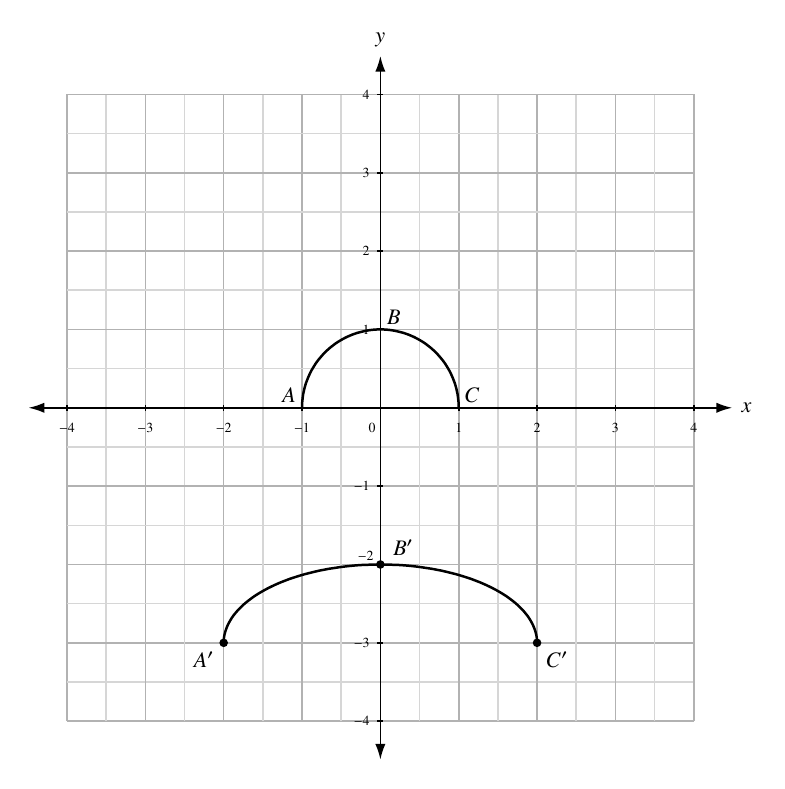
\begin{tikzpicture}[x=0.0127cm, y=-0.0127cm]
\draw[black!30] (54.5,78.5) -- (54.5,705.5);
\draw[black!30] (54.5,705.5) -- (681.5,705.5);
\draw[black!16] (93.7,78.5) -- (93.7,705.5);
\draw[black!16] (54.5,666.3) -- (681.5,666.3);
\draw[black!30] (132.9,78.5) -- (132.9,705.5);
\draw[black!30] (54.5,627.1) -- (681.5,627.1);
\draw[black!16] (172.1,78.5) -- (172.1,705.5);
\draw[black!16] (54.5,587.9) -- (681.5,587.9);
\draw[black!30] (211.2,78.5) -- (211.2,705.5);
\draw[black!30] (54.5,548.8) -- (681.5,548.8);
\draw[black!16] (250.4,78.5) -- (250.4,705.5);
\draw[black!16] (54.5,509.6) -- (681.5,509.6);
\draw[black!30] (289.6,78.5) -- (289.6,705.5);
\draw[black!30] (54.5,470.4) -- (681.5,470.4);
\draw[black!16] (328.8,78.5) -- (328.8,705.5);
\draw[black!16] (54.5,431.2) -- (681.5,431.2);
\draw[black!30] (368.0,78.5) -- (368.0,705.5);
\draw[black!30] (54.5,392.0) -- (681.5,392.0);
\draw[black!16] (407.2,78.5) -- (407.2,705.5);
\draw[black!16] (54.5,352.8) -- (681.5,352.8);
\draw[black!30] (446.4,78.5) -- (446.4,705.5);
\draw[black!30] (54.5,313.6) -- (681.5,313.6);
\draw[black!16] (485.6,78.5) -- (485.6,705.5);
\draw[black!16] (54.5,274.4) -- (681.5,274.4);
\draw[black!30] (524.8,78.5) -- (524.8,705.5);
\draw[black!30] (54.5,235.2) -- (681.5,235.2);
\draw[black!16] (563.9,78.5) -- (563.9,705.5);
\draw[black!16] (54.5,196.1) -- (681.5,196.1);
\draw[black!30] (603.1,78.5) -- (603.1,705.5);
\draw[black!30] (54.5,156.9) -- (681.5,156.9);
\draw[black!16] (642.3,78.5) -- (642.3,705.5);
\draw[black!16] (54.5,117.7) -- (681.5,117.7);
\draw[black!30] (681.5,78.5) -- (681.5,705.5);
\draw[black!30] (54.5,78.5) -- (681.5,78.5);
\draw[<->] (16,392) -- (720,392);
\draw[<->] (368,744) -- (368,40);
\draw (54.5,389) -- (54.5,395);
\draw (365,705.5) -- (371,705.5);
\node[font=\tiny, anchor=north, inner sep=0pt] at (54.5,407) {$-4$};
\node[font=\tiny, anchor=east, inner sep=0pt] at (358,705.5) {$-4$};
\draw (132.9,389) -- (132.9,395);
\draw (365,627.1) -- (371,627.1);
\node[font=\tiny, anchor=north, inner sep=0pt] at (132.9,407) {$-3$};
\node[font=\tiny, anchor=east, inner sep=0pt] at (358,627.1) {$-3$};
\draw (211.2,389) -- (211.2,395);
\draw (365,548.8) -- (371,548.8);
\node[font=\tiny, anchor=north, inner sep=0pt] at (211.2,407) {$-2$};
\node[font=\tiny, anchor=south east, inner sep=0pt] at (362,545.8) {$-2$};
\draw (289.6,389) -- (289.6,395);
\draw (365,470.4) -- (371,470.4);
\node[font=\tiny, anchor=north, inner sep=0pt] at (289.6,407) {$-1$};
\node[font=\tiny, anchor=east, inner sep=0pt] at (358,470.4) {$-1$};
\draw (446.4,389) -- (446.4,395);
\draw (365,313.6) -- (371,313.6);
\node[font=\tiny, anchor=north, inner sep=0pt] at (446.4,407) {$1$};
\node[font=\tiny, anchor=east, inner sep=0pt] at (358,313.6) {$1$};
\draw (524.8,389) -- (524.8,395);
\draw (365,235.2) -- (371,235.2);
\node[font=\tiny, anchor=north, inner sep=0pt] at (524.8,407) {$2$};
\node[font=\tiny, anchor=east, inner sep=0pt] at (358,235.2) {$2$};
\draw (603.1,389) -- (603.1,395);
\draw (365,156.9) -- (371,156.9);
\node[font=\tiny, anchor=north, inner sep=0pt] at (603.1,407) {$3$};
\node[font=\tiny, anchor=east, inner sep=0pt] at (358,156.9) {$3$};
\draw (681.5,389) -- (681.5,395);
\draw (365,78.5) -- (371,78.5);
\node[font=\tiny, anchor=north, inner sep=0pt] at (681.5,407) {$4$};
\node[font=\tiny, anchor=east, inner sep=0pt] at (358,78.5) {$4$};
\node[font=\tiny, anchor=north east, inner sep=0pt] at (364,407) {$0$};
\node[font=\footnotesize, anchor=west, inner sep=2pt] at (722,392) {$x$};
\node[font=\footnotesize, anchor=south, inner sep=2pt] at (368,38) {$y$};
\draw[line width=0.9pt] plot[smooth] coordinates {(289.6,392.0) (289.7,389.2) (289.8,386.5) (290.1,383.7) (290.4,381.0) (290.8,378.2) (291.4,375.5) (292.0,372.8) (292.7,370.2) (293.5,367.5) (294.5,364.9) (295.5,362.3) (296.6,359.8) (297.7,357.3) (299.0,354.8) (300.4,352.4) (301.8,350.1) (303.3,347.7) (304.9,345.5) (306.6,343.3) (308.4,341.2) (310.2,339.1) (312.1,337.1) (314.1,335.1) (316.1,333.3) (318.2,331.5) (320.4,329.8) (322.6,328.1) (324.9,326.5) (327.2,325.1) (329.6,323.7) (332.0,322.4) (334.5,321.1) (337.1,320.0) (339.6,318.9) (342.2,318.0) (344.8,317.1) (347.5,316.4) (350.2,315.7) (352.9,315.1) (355.6,314.6) (358.3,314.2) (361.1,313.9) (363.9,313.7) (366.6,313.6) (369.4,313.6) (372.1,313.7) (374.9,313.9) (377.7,314.2) (380.4,314.6) (383.1,315.1) (385.8,315.7) (388.5,316.4) (391.2,317.1) (393.8,318.0) (396.4,318.9) (398.9,320.0) (401.5,321.1) (404.0,322.4) (406.4,323.7) (408.8,325.1) (411.1,326.5) (413.4,328.1) (415.6,329.8) (417.8,331.5) (419.9,333.3) (421.9,335.1) (423.9,337.1) (425.8,339.1) (427.6,341.2) (429.4,343.3) (431.1,345.5) (432.7,347.7) (434.2,350.1) (435.6,352.4) (437.0,354.8) (438.3,357.3) (439.4,359.8) (440.5,362.3) (441.5,364.9) (442.5,367.5) (443.3,370.2) (444.0,372.8) (444.6,375.5) (445.2,378.2) (445.6,381.0) (445.9,383.7) (446.2,386.5) (446.3,389.2) (446.4,392.0)};
\node[font=\footnotesize, anchor=south east, inner sep=1.5pt] at (288.6,392) {$A$};
\node[font=\footnotesize, anchor=south west, inner sep=1.5pt] at (369.0,313.6) {$B$};
\node[font=\footnotesize, anchor=south west, inner sep=1.5pt] at (447.4,392) {$C$};
\draw[line width=0.9pt] plot[smooth] coordinates {(211.2,627.1) (211.3,624.4) (211.6,621.6) (212.1,618.8) (212.8,616.1) (213.7,613.4) (214.8,610.6) (216.0,608.0) (217.5,605.3) (219.1,602.6) (220.9,600.0) (222.9,597.5) (225.1,594.9) (227.5,592.4) (230.0,590.0) (232.7,587.5) (235.6,585.2) (238.6,582.9) (241.8,580.6) (245.2,578.4) (248.7,576.3) (252.4,574.2) (256.2,572.2) (260.1,570.3) (264.2,568.4) (268.4,566.6) (272.8,564.9) (277.2,563.2) (281.8,561.7) (286.5,560.2) (291.2,558.8) (296.1,557.5) (301.1,556.3) (306.1,555.1) (311.2,554.1) (316.4,553.1) (321.7,552.3) (327.0,551.5) (332.3,550.8) (337.8,550.2) (343.2,549.7) (348.7,549.3) (354.2,549.1) (359.7,548.9) (365.2,548.8) (370.8,548.8) (376.3,548.9) (381.8,549.1) (387.3,549.3) (392.8,549.7) (398.2,550.2) (403.7,550.8) (409.0,551.5) (414.3,552.3) (419.6,553.1) (424.8,554.1) (429.9,555.1) (434.9,556.3) (439.9,557.5) (444.8,558.8) (449.5,560.2) (454.2,561.7) (458.8,563.2) (463.2,564.9) (467.6,566.6) (471.8,568.4) (475.9,570.3) (479.8,572.2) (483.6,574.2) (487.3,576.3) (490.8,578.4) (494.2,580.6) (497.4,582.9) (500.4,585.2) (503.3,587.5) (506.0,590.0) (508.5,592.4) (510.9,594.9) (513.1,597.5) (515.1,600.0) (516.9,602.6) (518.5,605.3) (520.0,608.0) (521.2,610.6) (522.3,613.4) (523.2,616.1) (523.9,618.8) (524.4,621.6) (524.7,624.4) (524.8,627.1)};
\node[pt] at (211.25,627.125) {}; \node[pt] at (368.0,548.75) {}; \node[pt] at (524.75,627.125) {};
\node[font=\footnotesize, anchor=north east, inner sep=3pt] at (211.25,627.125) {$A'$};
\node[font=\footnotesize, anchor=south west, inner sep=3pt] at (371.0,548.75) {$B'$};
\node[font=\footnotesize, anchor=north west, inner sep=3pt] at (524.75,627.125) {$C'$};
\end{tikzpicture}
\end{document}
